%%%%%%%%%%%%%%%%%%%%%%%%%%%%%%%%%%%%%%%%%%%%%%%%%%
%% Authors :    Giovanni Arcari                 %%
%%              Maria Bronzova                  %%
%%              Luca Sardi                      %%
%%              Spencer Sharp                   %%
%%                                              %%
%% Supervisor : Andreas Apostolatos             %%
%%											  	%%
%% e-mail : andreas.apostolatos@tum.de		   	%%
%%											  	%%
%% 05_Perturbation_study.tex				    %%
%%											  	%%
%%%%%%%%%%%%%%%%%%%%%%%%%%%%%%%%%%%%%%%%%%%%%%%%%%
\section{PERTURBATION STUDY} \label{section:perturbationstudy}
As shown throughout the previous sections, results in sensitivity analysis are also driven by the chosen value for the perturbation, which is used to approximate the derivatives in the finite differencing schemes.\\[3pt]
The aim of this section is to try to show the general error behavior, to make the reader conscious of how the simulation can be badly affected if the perturbation value is chosen without any attention.
\subsection{Error assessment for decreasing perturbation values}
First of all, for the sake of clarity, it's important to state what is meant by perturbation value: in fact, this represents the displacement of a node normalized by the length of the element in the accounted direction.\\[3pt]
It's important to remind how the value shown are related to the run analysis and don't hold for any case, and how the aim of the perturbation study is to show a generic trend. \\[3pt]
Here follows the procedure used to assess the error: first of all, a type of sensitivity analysis was chosen. In this case a displacement sensitivity was run first, later it was verified how the behavior - with different error value but a similar trend - holds for all the other analysis. \\[3pt]
Then, the value of the sensitivity at a designated node was taken and stored, the perturbation value changed and the analysis performed again. \\[3pt]
As error, the difference between the sensitivity from each analysis and the value to which it converged for decreasing values of perturbation is taken. The latter was deliberately rounded off in order not to have an exact zero value for the error, which could be misleading.\\[3pt]
Two differencing schemes - backward and central - are chosen.
By running the analysis, it was possible to get the following data, plotted here in a double logarithmic scale.
\begin{figure}[h]
\centering
  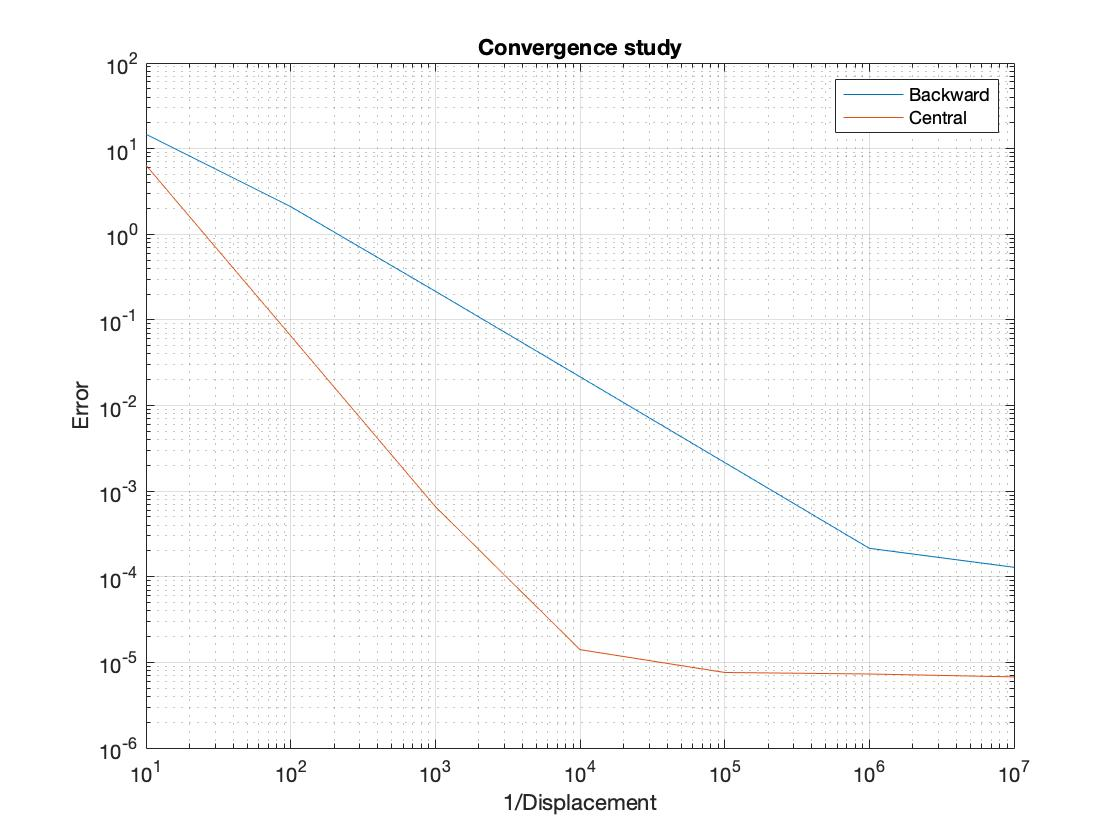
\includegraphics[width=140mm]{images/perturbation.jpg}
  \caption{Error assessment for decreasing perturbation values}
\end{figure}
\\[4pt] From this graph, it is possible to deduce some interesting information: first of all, the error decreases with twice the slope - in double logarithmic scale - for central differencing compared to backward and forward schemes, whose curve would overlap if both plotted. Then, it's noticeable how after a certain value, decreasing the perturbation does not lead to any change in the error: this is the range where a proper perturbation value can be chosen. \\[3pt]
Going further, it would be possible to see how the simulation blows up for perturbation value whose order of magnitude is around $10e-12$. This is due to the fact that the calculators are not able to represent any number, so at a certain level the results would just contain numerical waste.